\documentclass[12pt]{article}

\usepackage{amsfonts, amsmath, amssymb, amstext, latexsym}
\usepackage{graphicx, epsfig}
\usepackage[utf8]{inputenc}
\usepackage[french]{babel}
\usepackage[margin=1.0in]{geometry}
\usepackage{exscale}
\usepackage{amsbsy}
\usepackage{amsopn}
\usepackage{fancyhdr}
\usepackage{amsmath,amssymb}
\usepackage{graphicx}
\usepackage{subcaption}
%\usepackage{listings}
%\usepackage{textcomp}

\newcommand{\N}{\mathbb{N}}
\newcommand{\R}{\mathbb{R}}
\newcommand{\noi}{\noindent}
\newcommand{\dsp}{\displaystyle}
\newcommand{\iieme}{i^{\footnotesize \mbox{ème}}}
\newcommand{\jieme}{j^{\footnotesize \mbox{ème}}}
\newcommand{\jmunieme}{(j-1)^{\footnotesize \mbox{ème}}}
\newcommand{\dsum}[2]{\sum\limits_{#1}^{#2}}
\newcommand{\dprod}[2]{\prod\limits_{#1}^{#2}}

\def\ligne#1{\leaders\hrule height #1\linethickness \hfill}
% utilisation :
% \ligne{5}

\renewcommand{\theequation}{\thesection.\arabic{equation}}
\numberwithin{equation}{section}


\textheight 25cm
\textwidth 16cm
\oddsidemargin 0cm
\evensidemargin 0cm
\topmargin 0cm
\hoffset -0mm
\voffset -20mm

\pagestyle{plain}

\title{{Report TNCG15 }\\}

\author{Benjamin Palisse \\ Ikshu Dutta}
%\date{\today\\\currenttime}
\date{\today}

\begin{document}
\maketitle

\section{Abstract}
This paper presents a global illumination method, where the aim is to add light in a 3D scene to obtain a photo realistic effect. All the results are presented in a room which is rendered by using a Monte Carlo Ray Tracer. Rays are launched from the camera towards every pixel on the screen, and we compute the radiance at every intersection point between a ray and an object in the scene along with the global rendering equation. Russian Roulette is used to limit the recursion of the rays. The room is an open room that has 5 walls and 3 cubes, and all the objects in the scene are Lambertian reflectors. The room is lit up by using two area lights in the roof. This paper was produced for the course TNGC15, Global Illumination and Rendering, given by Mark E. Dieckman during the autumn of 2015.

\section{Introduction}

To compute the light inside a 3D scene, we need to compute the distribution of light energy within the scene. To do so, we will consider the radiance, because this quantity reveals the appearance of the objects [Advanced Global Illumination]. Ray tracing is mainly used to compute the radiance in the scene, but it is very time consuming. Different kind of ray tracers exist, for instance the Whitted ray tracer and the Monte Carlo ray tracer. Their differences lies in the way they compute the indirect illumination term of the global rendering equation. Once a ray hits a surface, the combined radiance of the objects around the surface is taken into account. To do this, more rays are sent from the intersection point towards the rest of the scene.\\
\\
In the Whitted ray tracer, 2 new rays are created: one in the specular reflection (see $figure 1$) and the other one in the refracted direction (see $figure 2$). Both of these directions are computed by the Snell-Descarte laws. This is well adapted for perfect specular and transparent objects. If the object is a diffuse object, the refracted ray is absorbed.
In the Monte-Carlo ray tracer, one or more rays are sent in a random direction toward the scene. This technique is good with Lambertian reflectors, which sends a perfect diffus light (see $figure 3$). To finish the recursion of rays created when a ray hit a surface, russian roulette is an efficient method: after every hit, a ray has a probability$\alpha$ to kill itself and so to not create more rays [russian roulette]. The use of a random depth gives a better approximation of the rendering equation, however, Monte Carlo Ray Tracing also gives noisy results. Ways to combat noise (and improve the approximation) is to use super sampling. A way to improve the results is to use a two pass rendering method, like photon mapping[article presentation].\\

\begin{figure}
  \begin{center}
    
\includegraphics[scale=0.6]{425px-ray_optics_diagram_incidence_reflection_and_refraction_svg_wide.png}
    \caption{a ray is reflected in the specular direction after hitting a mirror}
    \label{fig:1}
  \end{center}
\end{figure}

\begin{figure}
  \begin{center}
    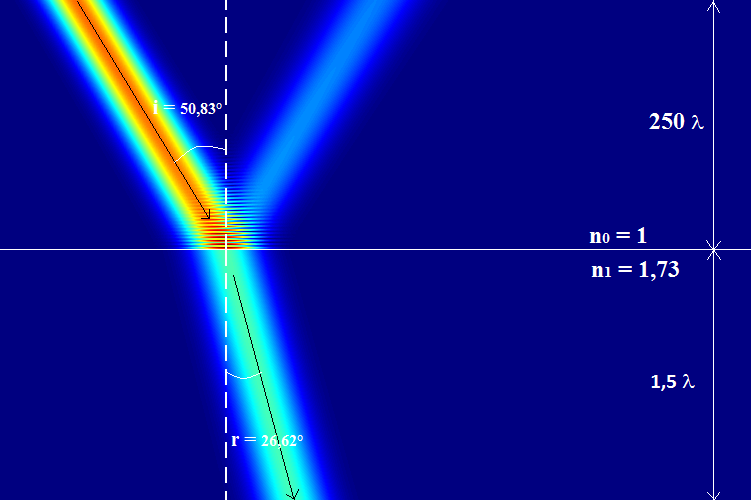
\includegraphics[scale=0.3]{RefractionModelisation.png}
    \caption{a ray is refracted, and a smaller part is reflected}
    \label{fig:2}
  \end{center}
\end{figure}

\begin{figure}
  \begin{center}
    \includegraphics[scale=2.0]{diffus.png}
    \caption{diffus light: it seems the same regardless of the observer's angle of view }
    \label{fig:3}
  \end{center}
\end{figure}

In a two pass rendering method, two photon maps are computed during the first pass: photons are emitted from the lights sources and are stored in these photon maps when they hit a surface. With this information, in the second pass, optimized sampling directions can be generated by ray tracing the scene. When a ray hits a surface, the photon map is used to give the information of the lighting of the scene. Moreover, the number of shadow rays inside the program can be greatly reduced by using the shadow photons, as they can be used to simulate shadows. Furthermore, one of the two photon maps allows to render caustic effect, which is normally very hard to render with a "normal" Monte Carlo ray tracer.\\


A use of a ray caster can be the detection of iso-surface[article]. Rays are cast from the camera toward every pixel and then go across the scene. We follow every ray with a step $dt$ and at every step, we compute the value of the data we are interested in. The aim is to find at which moment we will reach the isovalue. However, since we discretize the values along the ray, it is possible and even very probable that the values computed on the ray will never be exactly equal to the isosurface, even if the ray cross it. One solution is to reduced the step $dt$, but even so the isovalue could still be between two discret values of the ray, and the smaller $dt$ is, the more time the calculation take. So it is better to consider the difference $valueComputed - isovalue$. When the sign of this difference changes (the value on ray become bigger or smaller than the isovalue), we know we just cross an isosurface. Then, we can find more precisely where the isovalue is taken, by using a dichotomic algorithm or a reverse linear interpolation.\\

The first section is the introduction. In section 2, we will discuss the techniques like the Russian Roulette that we have implemented. The section 3 presents some results we obtained with our implementation. Then, in the section 4, we will explain how we can improve our renderer and the realism of our pictures. 

\section{Background}

\subsection{Intersection}

To compute the intersection between a ray and the objects in our room, the possible intersections the ray can collide with are computed, and the nearest one is determined. We proceed in a particular order when we check the obstacles in the room. First, we see if the ray intersects the object like sphere or cube in our room. Then, we check for the light sources, and finally for the wall. It's because in the way the room is built, it is not possible that a source light is positioned between a ray and a sphere/cube. So if there is an intersection between a ray and a sphere, we know that the sphere is the closest object the ray will intersect with. To find the intersection between a ray and a wall or a sphere, we inject the parametric equation of the ray inside the implicit equation of the wall or the sphere.\\


\subsection{Reflected rays}
Once a ray hits a surface, Russian Roulette is used to determine if the ray is terminated, or if it is reflected onto other surfaces. The rays have a probability of $\alpha$ to survive, and $1-\alpha$ to be terminated. If it bounces, then two angles are randomly created, $\theta$ and $\phi$. A fictive point is then created, which has the following spheric coordinates: $(r=1, \theta, \psi)$. We transform these coordinate into cartesian ones, and the new ray is directed toward this fictive point.

\subsection{Intensities}

\subsection{Shadow ray}

Every time a ray hit a surface, we need to compute how much radiance there is on this surface. To do so, we divide the incoming radiance in two parts, the direct lightings and the indirect lightings. For the direct part, we need to know if the intersection point receive light from the surface lights. To know that, we sample $n$ random points on the surface area, and then we create $n$ "shadow rays". These rays have the intersection point as origin, and are directed towards the sampled points on the light (figure $4$). We check then the intersections of the shadow rays with the room: if there are on the light, then we have a direct illumination. If there are not on the light, then there is an obstacle on the way and there is no direct illumination. It is possible that some of the shadow rays find a light and other don't. That's why we weighted the light given by the light source to the intersection point: if only half of shadow rays find a light source, then the contribution of this light source will be only half of what it would have been if all the shadow rays found the light source. We do that for every light inside the room. The result change along with the number $n$ of shadow rays.

\begin{figure}
  \begin{center}
    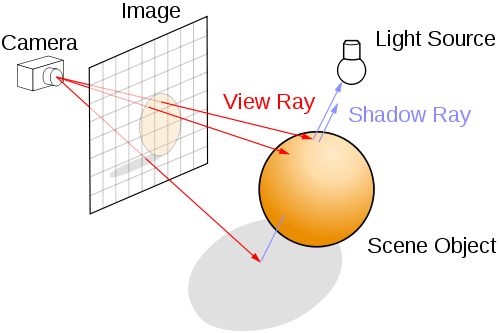
\includegraphics[scale=0.5]{500px-Ray_trace_diagram.png}
    \caption{once the ray hits the sphere, a shadow ray is sent toward the light source}
    \label{fig:4}
  \end{center}
\end{figure}

\section{Results and benchmarks}
Here are a serie of computations where we change one parameter at a time. The defaults parameters are the followings:
\begin{itemize}
\item Resolution: $500 \times 500$
\item Shadow Rays: 1
\item Sampling Rate: 8
\item Bounce Limit: 3

\end{itemize}
\subsection{Shadow rays}

The following pictures are generated with $1$, $4$, $20$, $50$ shadow rays. The figure ? presents the differents results obtained with a varying number of shadow rays.\\

    \begin{figure*}
        \centering
        \begin{subfigure}[b]{0.475\textwidth}
            \centering
            \includegraphics[width=\textwidth]{placeHolder.jpg}
            \caption[Network2]%
            {{\small 1 shadow ray}}    
            \label{fig:mean and std of net14}
        \end{subfigure}
        \hfill
        \begin{subfigure}[b]{0.475\textwidth}  
            \centering 
            \includegraphics[width=\textwidth]{placeHolder.jpg}
            \caption[]%
            {{\small 4 shadow rays}}    
            \label{fig:mean and std of net24}
        \end{subfigure}
        \vskip\baselineskip
        \begin{subfigure}[b]{0.475\textwidth}   
            \centering 
            \includegraphics[width=\textwidth]{placeHolder.jpg}
            \caption[]%
            {{\small 20 shadow rays}}    
            \label{fig:mean and std of net34}
        \end{subfigure}
        \quad
        \begin{subfigure}[b]{0.475\textwidth}   
            \centering 
            \includegraphics[width=\textwidth]{placeHolder.jpg}
            \caption[]%
            {{\small 50 shadow rays}}    
            \label{fig:mean and std of net44}
        \end{subfigure}
        \caption[  ]
        {\small Computation of the room by using a different number of shadow rays} 
        \label{fig:mean and std of nets}
    \end{figure*}


\begin{tabular}{| l | r |}
\hline
   number Shadow Ray & Time(s) \\
\hline
   1 & 61 \\
\hline
   4 & 164 \\
\hline
   16 & 556 \\
\hline   
   32 & 1024\\
\hline
 \end{tabular} 

\subsection{Resolution}

The figure ? presents the differents results obtained with a varying resolution.

    \begin{figure*}
        \centering
        \begin{subfigure}[b]{0.475\textwidth}
            \centering
            \includegraphics[width=\textwidth]{placeHolder.jpg}
            \caption[Resolution of 150 $\times$ 150]%
            {{\small Resolution of x $\times$ x}}    
            \label{fig:mean and std of net14}
        \end{subfigure}
        \hfill
        \begin{subfigure}[b]{0.475\textwidth}  
            \centering 
            \includegraphics[width=\textwidth]{placeHolder.jpg}
            \caption[]%
            {{\small Resolution of 300 $\times$ 300}}    
            \label{fig:mean and std of net24}
        \end{subfigure}
        \vskip\baselineskip
        \begin{subfigure}[b]{0.475\textwidth}   
            \centering 
            \includegraphics[width=\textwidth]{placeHolder.jpg}
            \caption[]%
            {{\small Resolution of 600 $\times$ 600}}    
            \label{fig:mean and std of net34}
        \end{subfigure}
        \quad
        \begin{subfigure}[b]{0.475\textwidth}   
            \centering 
            \includegraphics[width=\textwidth]{placeHolder.jpg}
            \caption[]%
            {{\small Resolution of 1200 $\times$ 1200}}    
            \label{fig:mean and std of net44}
        \end{subfigure}
        \caption[ The average and standard deviation of critical parameters ]
        {\small Computation of the room with differents resolution} 
        \label{fig:mean and std of nets}
    \end{figure*}

\begin{tabular}{| l | r |}
\hline
   Resolution & Time (s)\\
\hline
   150 $\times$ 150 & 44 \\
\hline
   300 $\times$ 300 & 173 \\
\hline
   600 $\times$ 600 & 704 \\
\hline   
   1200 $\times$ 1200 & 2796\\
\hline
 \end{tabular} 

\subsection{Sampling Rate}

It corresponds to the number of ray the camera sends to every pixel. The figure ? presents the differents results obtained with a varying sampling rate.

    \begin{figure*}
        \centering
        \begin{subfigure}[b]{0.475\textwidth}
            \centering
            \includegraphics[width=\textwidth]{placeHolder.jpg}
            \caption[Network2]%
            {{\small Sampling rate: 1}}    
            \label{fig:mean and std of net14}
        \end{subfigure}
        \hfill
        \begin{subfigure}[b]{0.475\textwidth}  
            \centering 
            \includegraphics[width=\textwidth]{placeHolder.jpg}
            \caption[]%
            {{\small Sampling rate: 8}}    
            \label{fig:mean and std of net24}
        \end{subfigure}
        \vskip\baselineskip
        \begin{subfigure}[b]{0.475\textwidth}   
            \centering 
            \includegraphics[width=\textwidth]{placeHolder.jpg}
            \caption[]%
            {{\small Sampling rate: 16}}    
            \label{fig:mean and std of net34}
        \end{subfigure}
        \quad
        \begin{subfigure}[b]{0.475\textwidth}   
            \centering 
            \includegraphics[width=\textwidth]{placeHolder.jpg}
            \caption[]%
            {{\small Sampling rate: 32}}    
            \label{fig:mean and std of net44}
        \end{subfigure}
        \caption[ The average and standard deviation of critical parameters ]
        {\small Computation of the room with different values for the sampling rate} 
        \label{fig:mean and std of nets}
    \end{figure*}

\begin{tabular}{| l | r |}
\hline
   Sampling Rate & Time \\
\hline
   1 & 23 \\
\hline
   8 & 164 \\
\hline
   16 & 324 \\
\hline   
   32 & 639\\
\hline
 \end{tabular} 

\subsection{Russian Roulette Probability}
We are going to modify the probability that a ray kills itself instead of bouncing. To have a better understanding of the impact of the modification of this value, we increase the maximum number of bounces that a ray can do: in this part, a ray can do until 20 bounces.  The figure ? presents the differents results obtained with a varying probability.
    \begin{figure*}
        \centering
        \begin{subfigure}[b]{0.475\textwidth}
            \centering
            \includegraphics[width=\textwidth]{placeHolder.jpg}
            \caption[Network2]%
            {{\small proba = 0.9}}    
            \label{fig:mean and std of net14}
        \end{subfigure}
        \hfill
        \begin{subfigure}[b]{0.475\textwidth}  
            \centering 
            \includegraphics[width=\textwidth]{placeHolder.jpg}
            \caption[]%
            {{\small proba = 0.5}}    
            \label{fig:mean and std of net24}
        \end{subfigure}
        \vskip\baselineskip
        \begin{subfigure}[b]{0.475\textwidth}   
            \centering 
            \includegraphics[width=\textwidth]{placeHolder.jpg}
            \caption[]%
            {{\small proba = 0.1}}    
            \label{fig:mean and std of net34}
        \end{subfigure}
        \quad
        \caption[ The average and standard deviation of critical parameters ]
        {\small Computation of the room with differents number of bounces} 
        \label{fig:mean and std of nets}
    \end{figure*}

\begin{tabular}{| l | r |}
\hline
   proba & Time \\
\hline
   0.9 & 134 \\
\hline
   0.5 & 164 \\
\hline
   0.1 & 266 \\
\hline 
 \end{tabular} 

\section{Discussion}

The program is a basic functional version of a Monte Carlo ray tracer, and a lot of features can be added to improve the realism. Oren-Nayor reflectors could be added at the scene. The walls will stay Lambertian reflectors, but the cubes should become Oren-Nayor reflectors. The object cube has an attribut BRDF which is a float initialized in its constructor. It should become a function of $(w_i, w_{out})$. Other features could be added, like the transparence of object, the photon maps. To increase the performance of our program, a better manager could be incorporated for the intersections: for now, the intersection between a ray and every object in the room is tested, even if the ray miss them from a lot. The problem could be resolved by putting the objects in an octree for instance.[wikipédia Octree] 


\section{Reference list}
\noindent [1] Philip Dutr\'e, Philippe Bekaert, Kavita Bala: "Advanced Global Illumination", 2002\\
$[2]$ Matt Pharr, Greg Humphreys: "Physically Based Rendering Second Edition" $2004$\\
$[3]$ Henrik Wann Jensen, "Global Illumination using Photon Maps" \\
$[4]$ Henrik Wann Jensen "A Practical Guide to Global Illumination using Photon Maps" Siggraph 2000 Course 8 Sunday, July 23, $2000$\\
$[5]$ https://fr.wikipedia.org/wiki/Octree\\



\nocite{*}
\bibliographystyle{plain}
\bibliography{biblio}
\end{document}
